\documentclass[9pt]{beamer}
\usetheme{Boadilla}
\usepackage{amsmath, textcmds, booktabs, graphicx}

\subtitle{Effects of Performance and Non-performance Factors on AAV of Free Agent contracts in Baseball}
\title{BTM301 Class Project}
\author[Team 1]{
    Onejune Lee,
    Minsoo Kang,
    Minwook Kim,
    Sunghun Ko
}
\institute{KAIST}
\date{\today}

\begin{document}
\begin{frame}
    \titlepage
\end{frame}
\begin{frame}
    \frametitle{Table of Contents}
    \tableofcontents
\end{frame}

\section{Introduction}
\begin{frame}
    \frametitle{Introduction}
    \begin{block}{Background}
        \begin{itemize}
            \item Free agent contracts in baseball are determined by various factors.
            \item It is clear that the salary of a player is not solely determined by performance.
            \item Non-performance factors that affects to salary can be thought as sort of \qq{bubble} or mispricing of market.
            \item Conversely, there may be some performance factors which are seemingly affecting the salary but actually not.
            \item To figure out the effects of these factors, we selected several factors, built a linear model based on these factors, ran regression, and interpreted the results.
        \end{itemize}
    \end{block}
\end{frame}
\begin{frame}
    \frametitle{Introduction}
    \begin{block}{Factors considered}
        Following are the factors that are not determined by performance of each player:
        \begin{itemize}
            \item WR: Win rate of the player's last team before free agency
            \item Atd: Average attendance at home game of the player's last team before free agency
            \item SU: Last season's total salary of team the player signed with
            \item L: Dummy variable indicating left-handedness of the player
            \item AGE: Age of the player at the time of signing
        \end{itemize}
        These can be thought as candidates of potential \qq{bubble} factors.
    \end{block}
\end{frame}
\begin{frame}
    \frametitle{Introduction}
    \begin{block}{Factors considered - cont'd}
        For the performance factors, we chose the following for hitters:
        \begin{itemize}
            \item OBP: On-base percentage of the player
            \item SLG: Slugging percentage of the player
            \item HR: Home runs of the player
            \item PA: Plate appearances of the player
        \end{itemize}
        Two of these factors are ratios, and the other two are cumulative values. We also included the league's average values for ratio factors to see if relative performance is more important than absolute performance or not.
    \end{block}
    Our initial plan was including more factors and league average of them, too, but failed to find the data for them.
\end{frame}
\begin{frame}
    \frametitle{Introduction}
    \begin{block}{Factors considered - cont'd}
        For the performance factors, we chose the following for pitchers:
        \begin{itemize}
            \item ERA: Earned run average of the player
            \item WHIP: Walks plus hits per inning pitched of the player
            \item SO: Strikeouts of the player
            \item IP: Innings pitched of the player
        \end{itemize}
        Again, two of these factors are ratios, and the other two are cumulative values, and we included the league's average values for ratio factors.
    \end{block}
\end{frame}

\section{Model}

\begin{frame}
    \frametitle{Model}
    \begin{block}{Rationale}
        What we expect is that the average annual value (AAV) is proportional to the factors we mentioned. We can write this as, for hitters:
        \[
            AAV \propto WR, \, Atd, \, SU, \, \lambda^L \text{ (for some } \lambda), \, \frac{1}{AGE}, \, OBP, \, SLG, \, HR, \, PA, \, OBP_{\text{avg}}, \, SLG_{\text{avg}},
        \]
        although we do not know the degree of proportionality. As you can see, taking logarithm on both sides, we can write this as a linear model. We can do the same for pitchers, too.
    \end{block}
\end{frame}

\begin{frame}
    \frametitle{Model}
    \begin{block}{Hitter Model}
        \begin{align*}
            \log{AAV_{i}} &= \beta_{WR} \log{WR_{i}}
                + \beta_{Atd} \log{Atd_{i}} 
                + \beta_{SU} \log{SU_{i}}
                + \beta_{L} L
                + \beta_{AGE}\log{AGE_{i}} \\
                &+ \beta_{OBP}\log{OBP_{i}}
                + \beta_{SLG}\log{SLG_{i}}
                + \beta_{HR}\log{HR_{i}}
                + \beta_{PA}\log{PA_{i}} \\
                &+ \beta_{OBP_{avg}}\log{OBP_{\text{avg}}}
                + \beta_{SLG_{avg}}\log{SLG_{\text{avg}}}
                + \beta_{0} 
                + \varepsilon_{i}
        \end{align*}
    \end{block}
    \begin{block}{Pitcher Model}
        \begin{align*}
            \log{AAV_{i}} &= \beta_{WR} \log{WR_{i}}
                + \beta_{Atd} \log{Atd_{i}} 
                + \beta_{SU} \log{SU_{i}}
                + \beta_{L} L
                + \beta_{AGE}\log{AGE_{i}} \\
                &+ \beta_{ERA}\log{ERA_{i}}
                + \beta_{WHIP}\log{WHIP_{i}}
                + \beta_{SO}\log{SO_{i}}
                + \beta_{IP}\log{IP_{i}} \\
                &+ \beta_{ERA_{avg}}\log{ERA_{\text{avg}}}
                + \beta_{WHIP_{avg}}\log{WHIP_{\text{avg}}}
                + \beta_{0} 
                + \varepsilon_{i}
        \end{align*}
    \end{block}
\end{frame}

\section{Data}

\begin{frame}
    \frametitle{Data}
    \begin{block}
        {Data Collection}
        \begin{itemize}
            \item 2010-2019 free agent contracts from MLB and KBO were collected. More recent data were excluded because we were not sure about how to handle the COVID-19's effects.
            \item Performance data was collected from Baseball Reference and KBO's official website
            \item Attendance data was collected from ESPN and KBO's official website
            \item Salary data was collected from independent researcher's website
            \item Both KBO and MLB's AAV and salary data were normalized by CPI at December of the year of signing, by Korea and US, respectively.
        \end{itemize}
    \end{block}
\end{frame}

\begin{frame}
    \frametitle{Data}
    \begin{block}{Disclaimer}
        \begin{itemize}
            \item Data of those who failed to find a team were excluded.
            \item Players whose performance was empty for various reasons (e.g., came from other leagues, got injured) were also excluded.
            \item There may be a potential unknown issues with data which ocurred in the process of data collection.
        \end{itemize}
    \end{block}
\end{frame}

\section{Results}
\begin{frame}
    \frametitle{Results}
    \begin{block}{MLB Hitters}
        
    \end{block}
\end{frame}

\begin{frame}
    \frametitle{Results}
    \begin{block}{MLB Pitchers: Regression Results}
        \begin{table}[ht]
            \centering
            \begin{tabular}{lcccccc}
            \toprule
            Variable & Coeff. & Std. Err & t-value & $P > |t|$ \\
            \midrule
            const & 13.3743 & 2.949 & 4.535 & 0.000 \\
            Win\_Pct & 1.0601 & 0.285 & 3.725 & 0.000  \\
            Attendance & 0.3321 & 0.225 & 1.479 & 0.140  \\
            Age & -1.7899 & 0.349 & -5.131 & 0.000  \\
            Is\_Left\_Handed & 0.0188 & 0.073 & 0.257 & 0.797  \\
            New\_Team\_Payroll\_Prev\_Year & 0.1624 & 0.081 & 1.996 & 0.047 \\
            ERA & 0.0660 & 0.116 & 0.566 & 0.572 \\
            WHIP & -1.3626 & 0.256 & -5.330 & 0.000  \\
            SO & 0.5457 & 0.141 & 3.882 & 0.000  \\
            IP & 0.0896 & 0.140 & 0.642 & 0.521  \\
            ERA\_league & 0.7778 & 1.070 & 0.727 & 0.468  \\
            WHIP\_league & -3.2791 & 2.445 & -1.341 & 0.181  \\
            \bottomrule
            \end{tabular}
            \end{table}
    \end{block}
\end{frame}
\begin{frame}
    \frametitle{Results}
    \begin{block}{MLB Pitchers: Residuals}
        \centering
        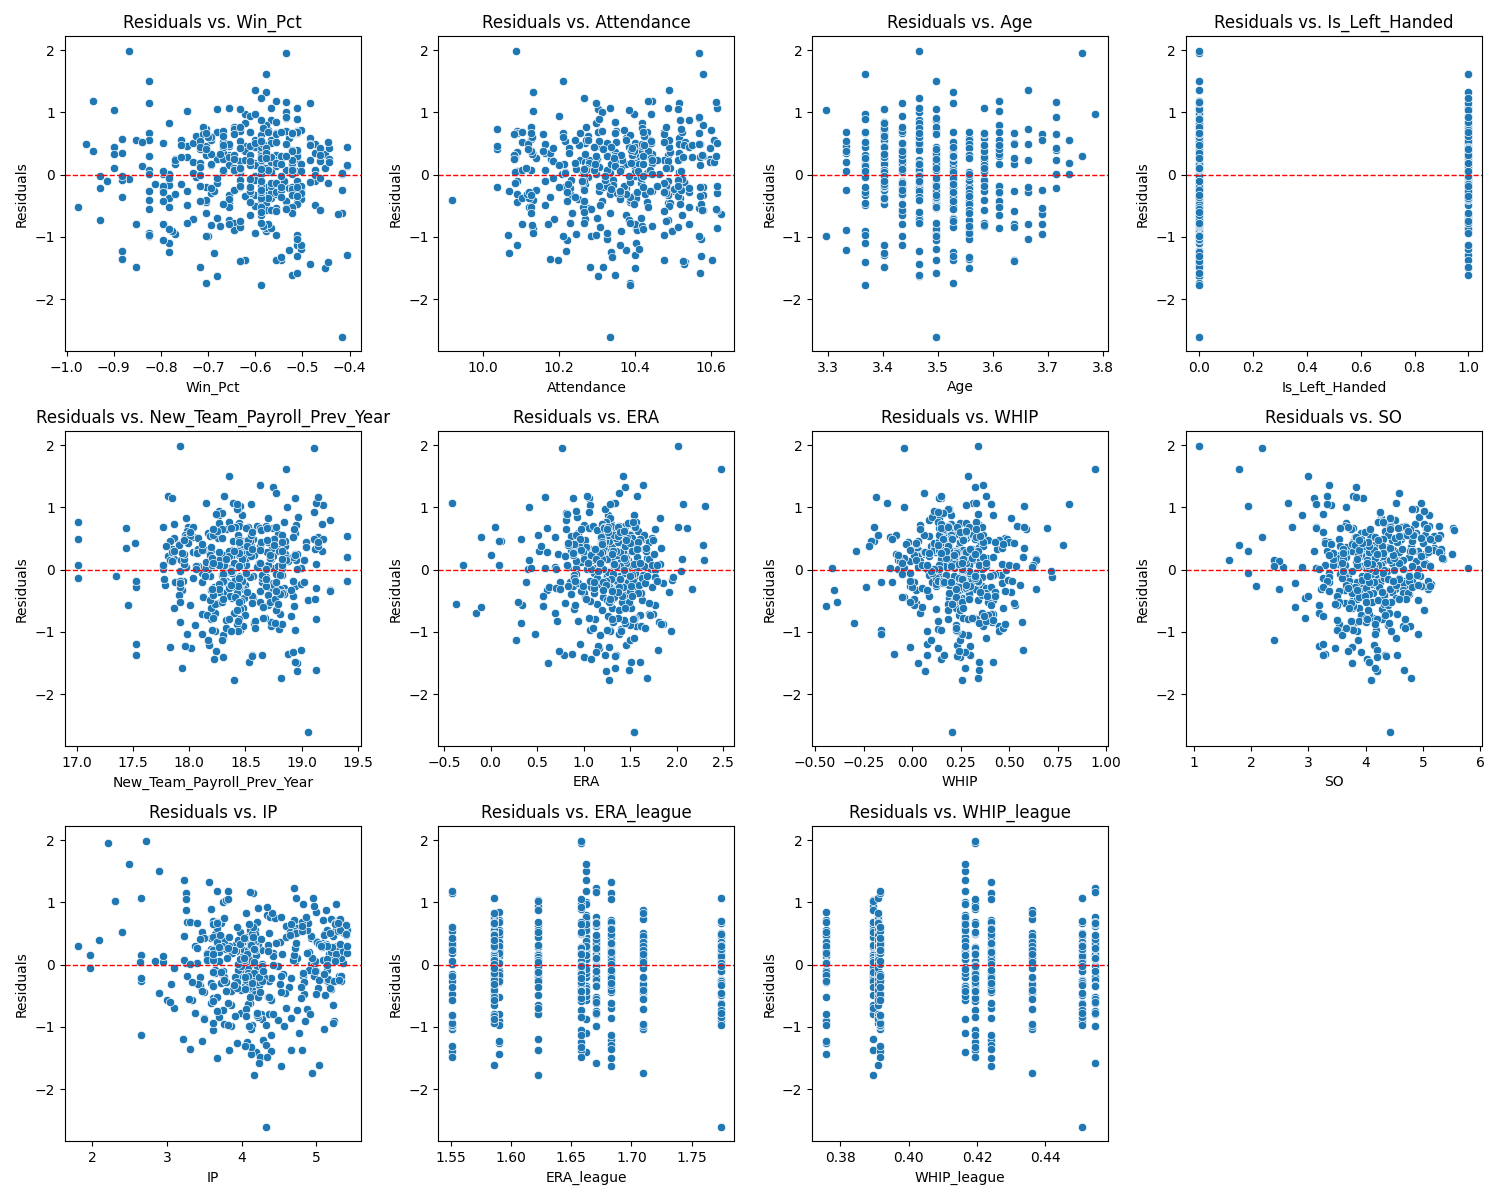
\includegraphics[height=0.75\textheight,keepaspectratio]{images/mlb_pitchers_residuals.png}
    \end{block}
\end{frame}

\begin{frame}
    \frametitle{Results}
    \begin{block}{KBO Hitters}
        
    \end{block}
\end{frame}

\begin{frame}
    \frametitle{Results}
    \begin{block}{KBO Pitchers}
        
    \end{block}
\end{frame}

\section{Discussion}
\begin{frame}
    \frametitle{Discussion}
\end{frame}

\section{Conclusion}
\begin{frame}
    \frametitle{Conclusion}
\end{frame}
\end{document}